\documentclass[SE,lsstdraft,authoryear,toc]{lsstdoc}
\input{meta}

% Package imports go here.
\usepackage{amsmath,amssymb,amsfonts}
% \usepackage{bm}  % incompatible with xelatex fonts; use \boldsymbol instead
\usepackage{booktabs}
\usepackage{tikz}
\usetikzlibrary{arrows.meta}

% Local commands go here.
\newcommand{\dd}{\mathrm{d}}
\newcommand{\Rix}{R_{ix}}
\newcommand{\Riy}{R_{iy}}

%If you want glossaries
%\input{aglossary.tex}
%\makeglossaries

\title{Rotator Rigid-Body Model Using LSSTCam Guider Sensors}

% This can write metadata into the PDF.
\hypersetup{
    pdftitle={Rotator Rigid-Body Model Using LSSTCam Guider Sensors},
    pdfauthor={Johnny H. Esteves},
    pdfkeywords={guider, rotator, rigid body, LSSTCam}
}

\input{authors}

\setDocRef{SITCOMTN-181}
\setDocUpstreamLocation{\url{https://github.com/lsst-sitcom/sitcomtn-181}}

\date{\vcsDate}

\setDocAbstract{%
We present the framework for extracting the rotator oscillation angle
$\delta\theta(t)$ from focal-plane centroid measurements of guide stars
tracked by the four corner guider sensors of LSSTCam.  The observed
centroid displacements are modelled as a rigid-body motion
(common-mode translation and rotation about the optical axis) plus
per-guider residuals from atmospheric and optical distortions.
Because the optics and atmospheric distortions are guider-dependent
and can impact our model, we estimate the rigid-body parameters using
a robust linear regression (M-estimator with iteratively reweighted
least squares).  We show that transforming to altitude/azimuth
coordinates via the local WCS Jacobian matrix at each guider position allows
a clean separation of the linear tracking drift from the
rigid-body motions.
}

% Change history defined here.
% Order: oldest first.
% Fields: VERSION, DATE, DESCRIPTION, OWNER NAME.
% See LPM-51 for version number policy.
\setDocChangeRecord{%
  \addtohist{1}{2026-03-21}{Initial version.}{Johnny H. Esteves}
}


\begin{document}

% Create the title page.
\maketitle

%======================================================================
\section{Setup and Coordinate System}
\label{sec:setup}

The LSSTCam focal plane uses a Cartesian coordinate system
$(x_\mathrm{fp}, y_\mathrm{fp})$ with origin at the instrument center
(Figure~\ref{fig:focalplane}).  Four corner raft positions host guider
sensors:

\begin{center}
\begin{tabular}{lcc}
\toprule
Corner Raft & Sensors & Nominal Position (mm) \\
\midrule
R00 (bottom-left)  & SG0, SG1 & $(-R_x,\;-R_y)$ \\
R04 (top-left)     & SG0, SG1 & $(-R_x,\;+R_y)$ \\
R40 (bottom-right) & SG0, SG1 & $(+R_x,\;-R_y)$ \\
R44 (top-right)    & SG0, SG1 & $(+R_x,\;+R_y)$ \\
\bottomrule
\end{tabular}
\end{center}

\noindent
Each individual sensor has its own guide star at a distinct focal-plane
position $(\Rix, \Riy)$ with lever arm
$R_i = \sqrt{\Rix^2 + \Riy^2}$.  These positions are all different in
general; we do \emph{not} assume equal radii.

\begin{figure}[ht!]
\centering
\begin{tikzpicture}[scale=0.022, >=Stealth]
  % Focal plane circle
  \draw[thick] (0,0) circle (320);

  % Center
  \fill (0,0) circle (3);
  \node[below right] at (5,-5) {$O$};

  % Corner guiders
  \fill[blue!70!black] (220,220) circle (5);
  \node[above right, blue!70!black] at (225,225) {R44};

  \fill[blue!70!black] (-220,220) circle (5);
  \node[above left, blue!70!black] at (-225,225) {R04};

  \fill[blue!70!black] (-220,-220) circle (5);
  \node[below left, blue!70!black] at (-225,-225) {R00};

  \fill[blue!70!black] (220,-220) circle (5);
  \node[below right, blue!70!black] at (225,-225) {R40};

  % Axes
  \draw[->, thick] (-350,0) -- (370,0) node[right] {$x_\mathrm{fp}$};
  \draw[->, thick] (0,-350) -- (0,370) node[above] {$y_\mathrm{fp}$};

  % Rotation arrow
  \draw[->, thick, red!70!black] (60,0) arc[start angle=0, end angle=70, radius=60];
  \node[red!70!black] at (85,50) {$\delta\theta$};

  % Radial line to R44
  \draw[dashed, gray] (0,0) -- (220,220);
  \node[gray, above] at (130,100) {$R_i$};

  % Tangential arrow at R44
  \draw[->, thick, orange!80!black] (220,220) -- (180,260);
  \node[orange!80!black, above left] at (175,265) {$\hat{t}_i$};
\end{tikzpicture}
\caption{LSSTCam focal plane showing the four corner guider rafts
(blue dots), the rotation angle $\delta\theta$ (red), and the
tangential direction $\hat{t}_i$ at corner R44 (orange).}
\label{fig:focalplane}
\end{figure}

%======================================================================
\section{Displacement Model}
\label{sec:model}

The observed centroid displacement of guide star $i$ at time $t$,
relative to its nominal focal-plane position $(\Rix, \Riy)$, has three
contributions:

\begin{equation}
\boxed{
\begin{aligned}
\delta x_i(t) &= \underbrace{dx(t)}_{\text{common translation}}
  - \underbrace{\delta\theta(t)\;\Riy}_{\text{rotation}}
  + \underbrace{\eta_{x_i}(t)}_{\text{atmosphere + noise}} \\[4pt]
\delta y_i(t) &= \underbrace{dy(t)}_{\text{common translation}}
  + \underbrace{\delta\theta(t)\;\Rix}_{\text{rotation}}
  + \underbrace{\eta_{y_i}(t)}_{\text{atmosphere + noise}}
\end{aligned}
}
\label{eq:displacement}
\end{equation}

\noindent
where:
\begin{itemize}
\item $dx(t),\; dy(t)$ is the common-mode translation from pointing
  errors, wind shake, mount jitter, and tracking drift.

\item $\delta\theta(t)$ is the rotation about the optical axis (rotator
  oscillation).

\item $\eta_{x_i}(t),\; \eta_{y_i}(t)$ are per-guider residuals.
  These include atmospheric tip-tilt (which is decorrelated across the
  ${\sim}\,440$\,mm guider separations), differential chromatic
  refraction, field-dependent optical distortions, and centroid
  measurement noise.  These terms are \emph{not} common-mode and
  cannot be described by the rigid-body model.
\end{itemize}

The rigid-body parameters $(dx, dy, \delta\theta)$ are common to all
guiders at each time step.  The per-guider residuals $\eta_i$ act as
effective noise in their estimation.  Because the optics and
atmospheric contributions can be large and variable across the focal
plane, they motivate the use of a robust estimator
(Section~\ref{sec:robust}).

\subsection{Per-Frame Linear System}
\label{sec:perframe}

At each time step, the $2N$ scalar displacement measurements from $N$
guide stars are related to the parameter vector
$\mathbf{p} = (dx,\; dy,\; \delta\theta)^T$ by:
\begin{equation}
\mathbf{A}\,\mathbf{p} = \mathbf{d} - \symbf{\eta}
\end{equation}
where the design matrix is:
\begin{equation}
\mathbf{A} =
\begin{pmatrix}
1 & 0 & -R_{1y} \\
0 & 1 & +R_{1x} \\
1 & 0 & -R_{2y} \\
0 & 1 & +R_{2x} \\
\vdots & \vdots & \vdots \\
1 & 0 & -R_{Ny} \\
0 & 1 & +R_{Nx}
\end{pmatrix},
\qquad
\mathbf{d} =
\begin{pmatrix}
\delta x_1 \\ \delta y_1 \\
\delta x_2 \\ \delta y_2 \\
\vdots \\
\delta x_N \\ \delta y_N
\end{pmatrix}
\label{eq:designmatrix_fp}
\end{equation}

\noindent
This is a $(2N \times 3)$ overdetermined system per frame.

\subsection{Per-Star Rotation Estimate}
\label{sec:perstar}

For geometric intuition, the per-star rotation estimate is:
\begin{equation}
\delta\theta_i
= \frac{\Rix\,\delta y_i - \Riy\,\delta x_i}{\Rix^2 + \Riy^2}
= \frac{\delta t_i}{R_i}
\label{eq:dtheta_i}
\end{equation}
where $\delta t_i$ is the tangential displacement and $R_i$ is the
lever arm for star $i$.  Under the rigid-body model, each per-star
estimate is contaminated by translation:
\begin{equation}
\delta\theta_i
= \delta\theta
+ \frac{-\Riy\,dx + \Rix\,dy}{R_i^2}
+ \frac{\Rix\,\eta_{y_i} - \Riy\,\eta_{x_i}}{R_i^2}
\label{eq:dtheta_i_contam}
\end{equation}

\noindent
The translation contamination term differs for each star because the
positions $(\Rix, \Riy)$ and lever arms $R_i$ are all different.  It
cancels in the mean only under exact symmetry conditions
($\sum \Rix/R_i^2 = \sum \Riy/R_i^2 = 0$), which are not strictly
satisfied for real guide star positions.  This is why a joint fit of
all three parameters is preferable to averaging individual
$\delta\theta_i$ values.

%======================================================================
\section{Working in Alt/Az Coordinates}
\label{sec:altaz}

The common-mode translation $dx(t), dy(t)$ in focal-plane coordinates
contains contributions from multiple sources: mount jitter, wind
shake, and alt/az tracking drift.  Among these, the tracking drift is
a smooth, slowly-varying sky motion that is best described in
altitude/azimuth coordinates.  However, the mapping from focal-plane
to alt/az is \emph{guider-dependent}: each sensor sits at a different
position and orientation on the focal plane, so the same sky motion
produces different $(\delta x_\mathrm{fp}, \delta y_\mathrm{fp})$
displacements for each guider.

\subsection{Local WCS Jacobian}
\label{sec:fp_to_altaz}

The conversion from focal-plane to sky coordinates at each guider
position is given by the local World Coordinate System (WCS).  For
small displacements, the WCS reduces to a linear transformation---the
Jacobian of the pixel-to-sky mapping evaluated at the guide star
position:
\begin{equation}
\begin{pmatrix}
\delta\mathrm{alt}_i \\ \delta\mathrm{az}_i
\end{pmatrix}
= \mathbf{J}_i
\begin{pmatrix}
\delta x_{\mathrm{fp},i} \\ \delta y_{\mathrm{fp},i}
\end{pmatrix}
\label{eq:wcs_transform}
\end{equation}

\noindent
where $\mathbf{J}_i$ is the $2\times 2$ WCS Jacobian matrix (the CD
matrix in FITS convention, not the determinant) evaluated at the
position of guider $i$.  It
encodes:
\begin{enumerate}
\item The \textbf{plate scale} (${\sim}\,20\;\mathrm{arcsec/mm}$),
  approximately common but with field-dependent corrections from the
  optical distortion model.
\item The \textbf{local position angle}, set by the orientation of the
  sky coordinate axes relative to the focal-plane axes at the sensor
  position.  This depends on the rotator angle and the sensor's
  field position (each sensor has a different WCS orientation).
\item \textbf{Optical distortions} (the non-conformal part of the
  astrometric solution), which introduce differential scale and
  small skew terms beyond a pure rotation.
\end{enumerate}

\noindent
Each $\mathbf{J}_i$ can be computed from the astrometric solution
(e.g.\ the FITS WCS headers), or calibrated empirically from guider
data since both focal-plane and alt/az displacements are recorded.

\subsection{Two Types of Common-Mode Translation}
\label{sec:two_types}

Applying $\mathbf{J}_i$ to the focal-plane model
(Eq.~\ref{eq:displacement}), the displacement of guide star $i$ in
alt/az is:
\begin{equation}
\begin{pmatrix}
\delta\mathrm{alt}_i \\[2pt] \delta\mathrm{az}_i
\end{pmatrix}
= \mathbf{J}_i
\begin{pmatrix} dx \\ dy \end{pmatrix}
+ \delta\theta\;\mathbf{J}_i
\begin{pmatrix} -\Riy \\ +\Rix \end{pmatrix}
+ \mathbf{J}_i\,\symbf{\eta}_i
\label{eq:altaz_full}
\end{equation}

\noindent
This reveals an important subtlety.  In focal-plane coordinates, the
common-mode translation $(dx, dy)$ is identical for all guiders---it
captures rigid-body motions of the instrument (rotator lateral shift,
flexure).  However, the term $\mathbf{J}_i(dx, dy)^T$ is \emph{not}
common in alt/az because each guider has a different $\mathbf{J}_i$.
Conversely, a pure sky translation
$(\delta\mathrm{alt}_{\mathrm{cm}}, \delta\mathrm{az}_{\mathrm{cm}})$
that is common in alt/az (such as the tracking drift) maps to
\emph{different} focal-plane displacements
$\mathbf{J}_i^{-1}(\delta\mathrm{alt}_{\mathrm{cm}},
\delta\mathrm{az}_{\mathrm{cm}})^T$ for each guider.

We therefore distinguish two types of common-mode translation:
\begin{enumerate}
\item \textbf{Focal-plane common} (rotator lateral shift, instrument
  flexure, wind shake): the same $(dx, dy)$ for all guiders in
  focal-plane coordinates.  These are rigid-body motions of the
  instrument and are correctly captured by the per-frame model
  (Eq.~\ref{eq:displacement}).

\item \textbf{Sky-frame common} (tracking drift): a smooth sky motion
  $(\alpha\,t,\; \beta\,t)$ in alt/az that maps to a
  \emph{guider-dependent} focal-plane displacement via
  $\mathbf{J}_i^{-1}$.  This is not a rigid-body motion in the focal
  plane.
\end{enumerate}

\noindent
A model that works entirely in alt/az and assumes all translations are
common in that frame would misattribute focal-plane rigid-body motions
as non-common residuals, since a common $(dx, dy)$ in focal plane
produces slightly different $(\delta\mathrm{alt}, \delta\mathrm{az})$
for each guider (at the level of the off-diagonal variations in
$\mathbf{J}_i$, ${\sim}\,5\%$).

\emph{Remark.}  In practice, the off-diagonal terms of $\mathbf{J}_i$
are dominated by the local position angle rotation at each guider.
Since the position angles differ by only a few degrees across the
focal plane, the guider-dependent drift vectors in focal plane are
nearly parallel and thus nearly degenerate with a common $(dx, dy)$.
The non-rotational contributions (differential scale, optical
distortion shear) are much smaller.  Consequently, the practical
improvement of the hybrid model over a simple focal-plane fit with
post-hoc detrending is modest.

\subsection{Hybrid Model}
\label{sec:hybrid_model}

To correctly handle both types of translation, we adopt a
\textbf{hybrid approach}: the per-frame rigid-body fit operates in
focal-plane coordinates (where the instantaneous common translation is
truly common), while the linear tracking drift is modelled as an
alt/az sky motion that maps to each guider's focal plane through its
own $\mathbf{J}_i^{-1}$.

The full model for guider $i$ at time $t$ in focal-plane coordinates
is:
\begin{equation}
\boxed{
\begin{aligned}
\delta x_i(t) &= dx(t)
  + \bigl[\mathbf{J}_i^{-1}\bigr]_{x}\,
    \begin{pmatrix} \alpha_0 + \alpha\,t \\
                     \beta_0 + \beta\,t \end{pmatrix}
  - \delta\theta(t)\;\Riy
  + \eta_{x_i}(t) \\[4pt]
\delta y_i(t) &= dy(t)
  + \bigl[\mathbf{J}_i^{-1}\bigr]_{y}\,
    \begin{pmatrix} \alpha_0 + \alpha\,t \\
                     \beta_0 + \beta\,t \end{pmatrix}
  + \delta\theta(t)\;\Rix
  + \eta_{y_i}(t)
\end{aligned}
}
\label{eq:hybrid_model}
\end{equation}

\noindent
where:
\begin{itemize}
\item $dx(t),\; dy(t)$ is the oscillatory focal-plane common-mode
  translation (mount jitter, wind shake, flexure), fitted per frame.
\item $\alpha_0 + \alpha\,t,\; \beta_0 + \beta\,t$ is the
  linear tracking drift in alt/az, which maps to a
  \emph{guider-dependent} focal-plane displacement via
  $\mathbf{J}_i^{-1}$.
\item $\delta\theta(t)$ is the rotation, which may also contain a
  slow drift: $\delta\theta(t) = \theta_0 + \omega\,t +
  \widetilde{\delta\theta}(t)$.
\end{itemize}

\noindent
The \textbf{alt/az rotation lever arms} remain:
\begin{equation}
\begin{pmatrix} a_i \\ b_i \end{pmatrix}
= \mathbf{J}_i
\begin{pmatrix} -\Riy \\ +\Rix \end{pmatrix}
\label{eq:lever_def}
\end{equation}

\noindent
These are guider-dependent: they differ for each star because both
$\mathbf{J}_i$ and $(\Rix, \Riy)$ vary across the focal plane.  For
LSSTCam, the effective lever arms are
$|(a_i, b_i)| \approx 320$--$350$\,mm (reflecting the corner guider
distances from the optical axis).

%======================================================================
\section{Hybrid Estimation}
\label{sec:estimation}

Following the discussion in Section~\ref{sec:hybrid_model}, the
estimation proceeds in two steps: (1)~a global augmented fit for the
linear tracking drift, working in focal-plane coordinates with
per-guider $\mathbf{J}_i^{-1}$ mappings; and (2)~per-frame robust
fits of the residuals using the standard focal-plane design matrix.

\subsection{Per-Frame Linear System (Focal Plane)}

At each time step, the $2N$ focal-plane displacement measurements are
related to the parameter vector
$\mathbf{p} = (dx,\; dy,\; \delta\theta)^T$ by:
\begin{equation}
\mathbf{A}\,\mathbf{p} = \mathbf{d} - \symbf{\eta}
\end{equation}
where the design matrix is the standard focal-plane form
(Eq.~\ref{eq:designmatrix_fp}):
\begin{equation}
\mathbf{A}_{\mathrm{fp}} =
\begin{pmatrix}
1 & 0 & -R_{1y} \\
0 & 1 & +R_{1x} \\
\vdots & \vdots & \vdots \\
1 & 0 & -R_{Ny} \\
0 & 1 & +R_{Nx}
\end{pmatrix},
\qquad
\mathbf{d} =
\begin{pmatrix}
\delta x_1 \\ \delta y_1 \\
\vdots \\
\delta x_N \\ \delta y_N
\end{pmatrix}
\label{eq:designmatrix_fp2}
\end{equation}

\noindent
The first two columns extract the common-mode translation (identical
for all guiders in focal-plane coordinates); the third column extracts
$\delta\theta$ via the focal-plane lever arms $(-\Riy, +\Rix)$.

\subsection{Incorporating the Linear Tracking Drift}
\label{sec:augmented}

The linear tracking drift is a sky motion in alt/az, but we
incorporate it into the focal-plane system by mapping it to each
guider's focal plane through $\mathbf{J}_i^{-1}$.  The augmented
parameter vector is:
\begin{equation}
\mathbf{p}_{\mathrm{trend}}
= \bigl(\alpha_0,\;\alpha,\;
         \beta_0,\;\beta,\;
         \theta_0,\;\omega\bigr)^T
\label{eq:ptrend}
\end{equation}

\noindent
where $(\alpha_0, \alpha)$ and $(\beta_0, \beta)$ are
the intercept and drift rate of the tracking error in altitude and
azimuth, respectively.

For star $i$ at time $t_k$, denoting
$\mathbf{J}_i^{-1} = \bigl(\begin{smallmatrix} c_{i,00} & c_{i,01}
\\ c_{i,10} & c_{i,11} \end{smallmatrix}\bigr)$, the two rows of the
augmented design matrix $\widetilde{\mathbf{A}}$ are:
\begin{equation}
\widetilde{\mathbf{A}}_{ik} =
\begin{pmatrix}
c_{i,00} & c_{i,00}\,t_k & c_{i,01} & c_{i,01}\,t_k & -\Riy & -\Riy\,t_k \\
c_{i,10} & c_{i,10}\,t_k & c_{i,11} & c_{i,11}\,t_k & +\Rix & +\Rix\,t_k
\end{pmatrix}
\label{eq:augmented_A}
\end{equation}

\noindent
The first four columns encode the tracking drift mapped to the focal
plane of each guider via $\mathbf{J}_i^{-1}$, and the last two
columns encode the rotation trend.  Crucially, the coefficients
$c_{i,jk}$ \emph{vary across guiders}---the off-diagonal terms of
$\mathbf{J}_i^{-1}$ flip sign between left and right rafts
(${\sim}\,5\%$ of the diagonal), providing the leverage to separate
the alt/az drift from focal-plane rigid-body motions.

Stacking over all $N$ stars and $T$ frames gives a
$(2NT \times 6)$ system:
\begin{equation}
\widetilde{\mathbf{A}}\;\mathbf{p}_{\mathrm{trend}}
= \widetilde{\mathbf{d}} - \widetilde{\symbf{\eta}}
\label{eq:augmented_system}
\end{equation}

\noindent
A robust fit of this system (Section~\ref{sec:robust}) yields the six
trend parameters simultaneously.

\subsection{Per-Frame Residual Fit}
\label{sec:perframe_resid}

For each frame $k$, the trend prediction for guider $i$ is subtracted
in focal-plane coordinates:
\begin{equation}
\mathbf{r}_{i,k} =
\begin{pmatrix} \delta x_i \\ \delta y_i \end{pmatrix}_{\!\!k}
- \mathbf{J}_i^{-1}
  \begin{pmatrix}
  \alpha_0 + \alpha\,t_k \\
  \beta_0 + \beta\,t_k
  \end{pmatrix}
- \begin{pmatrix}
  -\Riy \\ +\Rix
  \end{pmatrix}
  (\theta_0 + \omega\,t_k)
\label{eq:trend_residuals}
\end{equation}

\noindent
Note that the trend subtraction is \emph{guider-dependent} because
each guider has its own $\mathbf{J}_i^{-1}$.  The stacked residuals
$\mathbf{r}_k$ are then fit with the standard focal-plane design
matrix $\mathbf{A}_{\mathrm{fp}}$ robustly:
\begin{equation}
\mathbf{A}_{\mathrm{fp}}\,\widetilde{\mathbf{p}}_k = \mathbf{r}_k
\end{equation}
yielding the detrended oscillatory parameters
$(dx_k,\; dy_k,\; \widetilde{\delta\theta}_k)$ at each time step.
These are now truly focal-plane common-mode motions, free of the
tracking drift.

%======================================================================
\section{Robust Estimation}
\label{sec:robust}

\subsection{Motivation}

The per-guider residuals $\eta_i$ can exhibit:
\begin{itemize}
\item Badly defined PSFs driven by turbulence or optical distortions
\item Occasional large outliers from saturated stars, poor PSF fits,
  or star trails
\item Guider-to-guider variance differences (heteroscedasticity),
  arising from differences in guide star brightness, SNR, and PSF
  quality across the four corners
\end{itemize}
Under these conditions, OLS gives excessive weight to outlier
measurements, biasing the rigid-body solution.

\subsection{M-Estimator via IRLS}

We replace the OLS $\ell_2$ loss with a robust loss function
$\rho(r)$ and solve:
\begin{equation}
\hat{\mathbf{p}} = \arg\min_{\mathbf{p}}
\sum_{j=1}^{2N} \rho\!\left(\frac{r_j}{\hat{\sigma}}\right)
\label{eq:mestimator}
\end{equation}
where $r_j = (\mathbf{A}\mathbf{p} - \mathbf{d})_j$ are the
residuals, $\hat{\sigma}$ is a robust scale estimate, and $\rho$ is a
bounded-influence loss function.

This is solved by \textbf{iteratively reweighted least squares (IRLS)}:
at each iteration $k$, compute weights from the current residuals and
solve the weighted least-squares problem:
\begin{equation}
\hat{\mathbf{p}}^{(k+1)}
= (\mathbf{A}^T \mathbf{W}^{(k)} \mathbf{A})^{-1}\,
  \mathbf{A}^T \mathbf{W}^{(k)} \mathbf{d}
\label{eq:irls}
\end{equation}
where $\mathbf{W}^{(k)} = \mathrm{diag}(w_1^{(k)}, \ldots,
w_{2N}^{(k)})$ with weights $w_j^{(k)} = \psi(r_j^{(k)} /
\hat{\sigma}) / (r_j^{(k)} / \hat{\sigma})$ and
$\psi = \rho'$ is the influence function.

We adopt \textbf{Tukey's bisquare} (biweight) loss:
\begin{equation}
\rho(u) =
\begin{cases}
\dfrac{c^2}{6}\left[1 - \left(1 - \dfrac{u^2}{c^2}\right)^{\!3}\right]
  & |u| \leq c \\[6pt]
\dfrac{c^2}{6} & |u| > c
\end{cases}
\label{eq:tukey}
\end{equation}
with the standard tuning constant $c = 4.685$, which gives 95\%
asymptotic efficiency relative to OLS under Gaussian errors while
completely rejecting gross outliers (zero weight for
$|r_j| > c\,\hat{\sigma}$).

The robust scale $\hat{\sigma}$ is estimated from the residuals using
the MAD (median absolute deviation):
\begin{equation}
\hat{\sigma} = 1.4826 \times \mathrm{median}\bigl(|r_j - \mathrm{median}(r_j)|\bigr)
\label{eq:mad}
\end{equation}
where the factor $1/\Phi^{-1}(3/4) \approx 1.4826$ is the
Gaussian-consistency factor, ensuring that $\hat{\sigma}$ equals the
standard deviation when the residuals are normally distributed.

\subsection{Algorithm Summary}

\begin{enumerate}
\item Initialise with OLS:
  $\hat{\mathbf{p}}^{(0)} = (\mathbf{A}^T\mathbf{A})^{-1}
  \mathbf{A}^T\mathbf{d}$.
\item Compute residuals $r_j^{(k)} = (\mathbf{A}\hat{\mathbf{p}}^{(k)}
  - \mathbf{d})_j$.
\item Estimate scale: $\hat{\sigma}^{(k)}$ via MAD
  (Eq.~\ref{eq:mad}).
\item Compute Tukey bisquare weights $w_j^{(k)}$.
\item Solve weighted least squares (Eq.~\ref{eq:irls}) for
  $\hat{\mathbf{p}}^{(k+1)}$.
\item Repeat steps 2--5 until convergence
  ($\|\hat{\mathbf{p}}^{(k+1)} - \hat{\mathbf{p}}^{(k)}\| < \epsilon$).
\end{enumerate}

\noindent
Convergence is typically reached in 3--5 iterations.  With $2N = 8$--16
observations and 3 parameters, each iteration is negligible in cost.

\subsection{Uncertainty Estimation}

The covariance of the robust estimator is approximately:
\begin{equation}
\mathrm{Cov}(\hat{\mathbf{p}})
\approx \hat{\sigma}^2\,
\frac{\frac{1}{2N}\sum \psi^2(r_j/\hat{\sigma})}
     {\left[\frac{1}{2N}\sum \psi'(r_j/\hat{\sigma})\right]^2}\;
(\mathbf{A}^T \mathbf{W} \mathbf{A})^{-1}
\label{eq:robust_cov}
\end{equation}

\noindent
This is an asymptotic approximation that does not fully account for
the bias introduced by clipping.  In practice we only use the
covariance as a rough diagnostic (e.g.\ to flag bad frames), not for formal inference.

For a simpler diagnostic, the robust RMS of $\delta\theta$ across
frames can be reported using the MAD:
\begin{equation}
\hat{\sigma}_{\delta\theta}
= 1.4826 \times \mathrm{MAD}(\widehat{\delta\theta}_{\,t})
\end{equation}

%======================================================================
\section{Application to dayObs 20230311, seqNum 73}
\label{sec:results}

The robust rigid-body decomposition was applied to a 30\,s $i$-band
guider exposure (dayObs 20230311, seqNum 73) using all 8 corner sensors
(R00, R04, R40, R44 $\times$ SG0, SG1).  The guider frame rate is
${\sim}\,4.5$\,Hz ($\Delta t \approx 0.22$\,s).

\subsection{Rotator Oscillation Characteristics}

The time series of $\delta\theta(t)$ (Figure~\ref{fig:dtheta_ts})
reveals a clear quasi-periodic oscillation with:
\begin{itemize}
\item \textbf{RMS amplitude:} $0.767''$
\item \textbf{Peak-to-peak:} ${\sim}\,4''$ (${\sim}\,2''$ semi-amplitude)
\item \textbf{Dominant period:} ${\sim}\,2$--$3$\,s (${\sim}\,0.3$--$0.5$\,Hz)
\item \textbf{Arc at focal plane:} the tangential displacement at the
  mean guider radius $\langle R_i \rangle = 333$\,mm is
  $\ell = \delta\theta\,\langle R_i \rangle$.  The arc RMSE is
  $0.025''$ (full) / $0.023''$ (detrended), with a peak-to-peak
  of $0.117''$.
\end{itemize}
The autocorrelation function shows a damped oscillatory structure,
consistent with the rotator servo hunting around its tracking setpoint.

\begin{figure}[ht!]
\centering
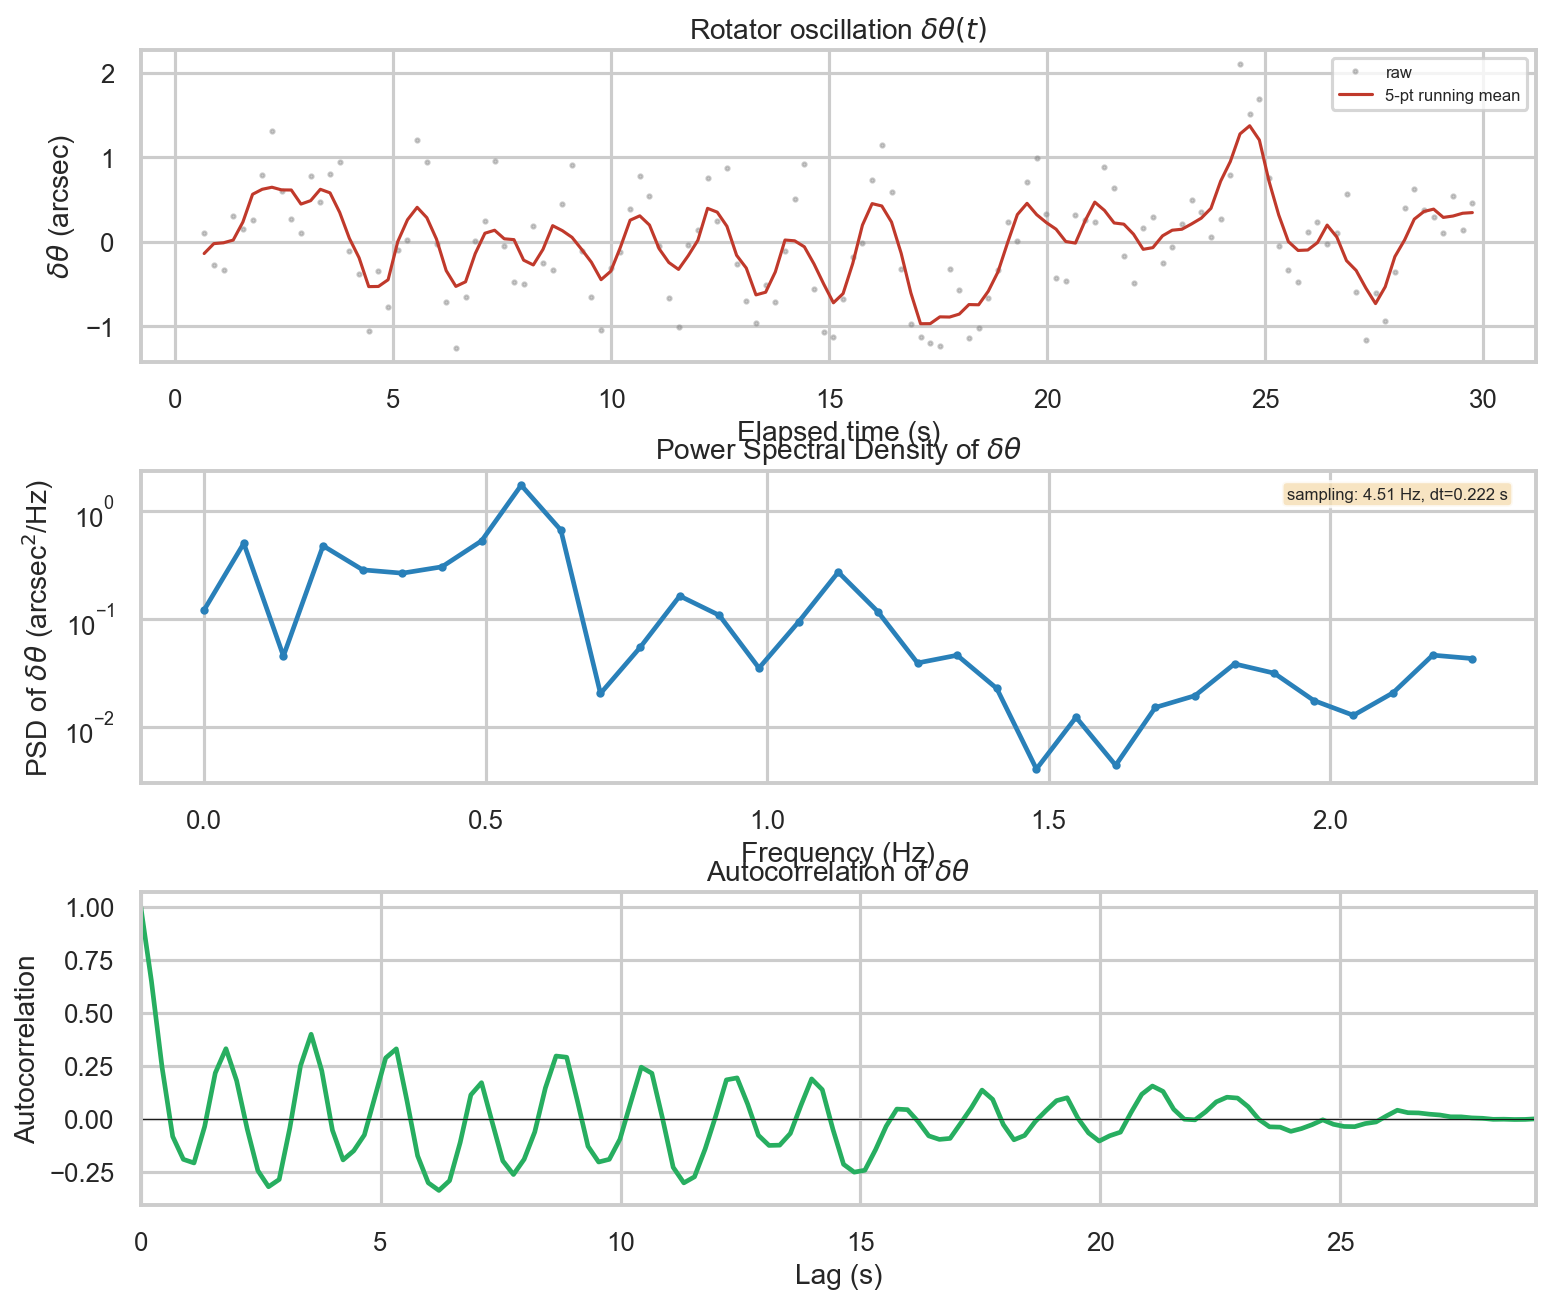
\includegraphics[width=0.95\textwidth]{dtheta_oscillation.png}
\caption{Top: $\delta\theta(t)$ time series (grey dots) with 5-point
running mean (red).  Middle: power spectral density.  Bottom:
autocorrelation function showing ${\sim}\,2$--$3$\,s periodicity.}
\label{fig:dtheta_ts}
\end{figure}

\subsection{Linear Tracking Drift}

The augmented fit (Section~\ref{sec:augmented}) yields the linear
drift rates directly as part of $\mathbf{p}_{\mathrm{trend}}$.  The
measured values are:

\begin{center}
\begin{tabular}{lrrr}
\toprule
\textbf{Parameter} & \textbf{Rate (arcsec/s)} & \textbf{Total over 30\,s (arcsec)} & \textbf{Arc $\ell$ (arcsec)} \\
\midrule
$\delta\mathrm{alt}$ & $-0.0037$ & $-0.111$ & --- \\
$\delta\mathrm{az}$  & $+0.0038$ & $+0.114$ & --- \\
$\delta\theta$        & $-0.0421$ & $-1.263$ & $0.041$ \\
\bottomrule
\end{tabular}
\end{center}

\noindent
Over the 30\,s exposure, the azimuth tracking drift accumulates to
$0.11''$, visible as the dominant linear slope in
Figure~\ref{fig:detrended} (panel~4).  The altitude drift contributes
$0.11''$, and the rotator drift $1.26''$.

Table~\ref{tab:detrended} compares the RMS before and after removing
the linear drift.

\begin{table}[ht!]
\centering
\caption{RMS before and after linear detrending.}
\label{tab:detrended}
\begin{tabular}{lrrr}
\toprule
& \textbf{Before detrending} & \textbf{After detrending} & \textbf{Arc $\ell$ RMS} \\
\textbf{Component} & \textbf{arcsec} & \textbf{arcsec} & \textbf{arcsec} \\
\midrule
$\delta\mathrm{alt}$  & 0.041 & 0.023 & --- \\
$\delta\mathrm{az}$   & 0.044 & 0.029 & --- \\
$\delta\theta$         & 0.767 & 0.725 & 0.025 / 0.023 \\
\bottomrule
\end{tabular}
\end{table}

\begin{figure}[ht!]
\centering
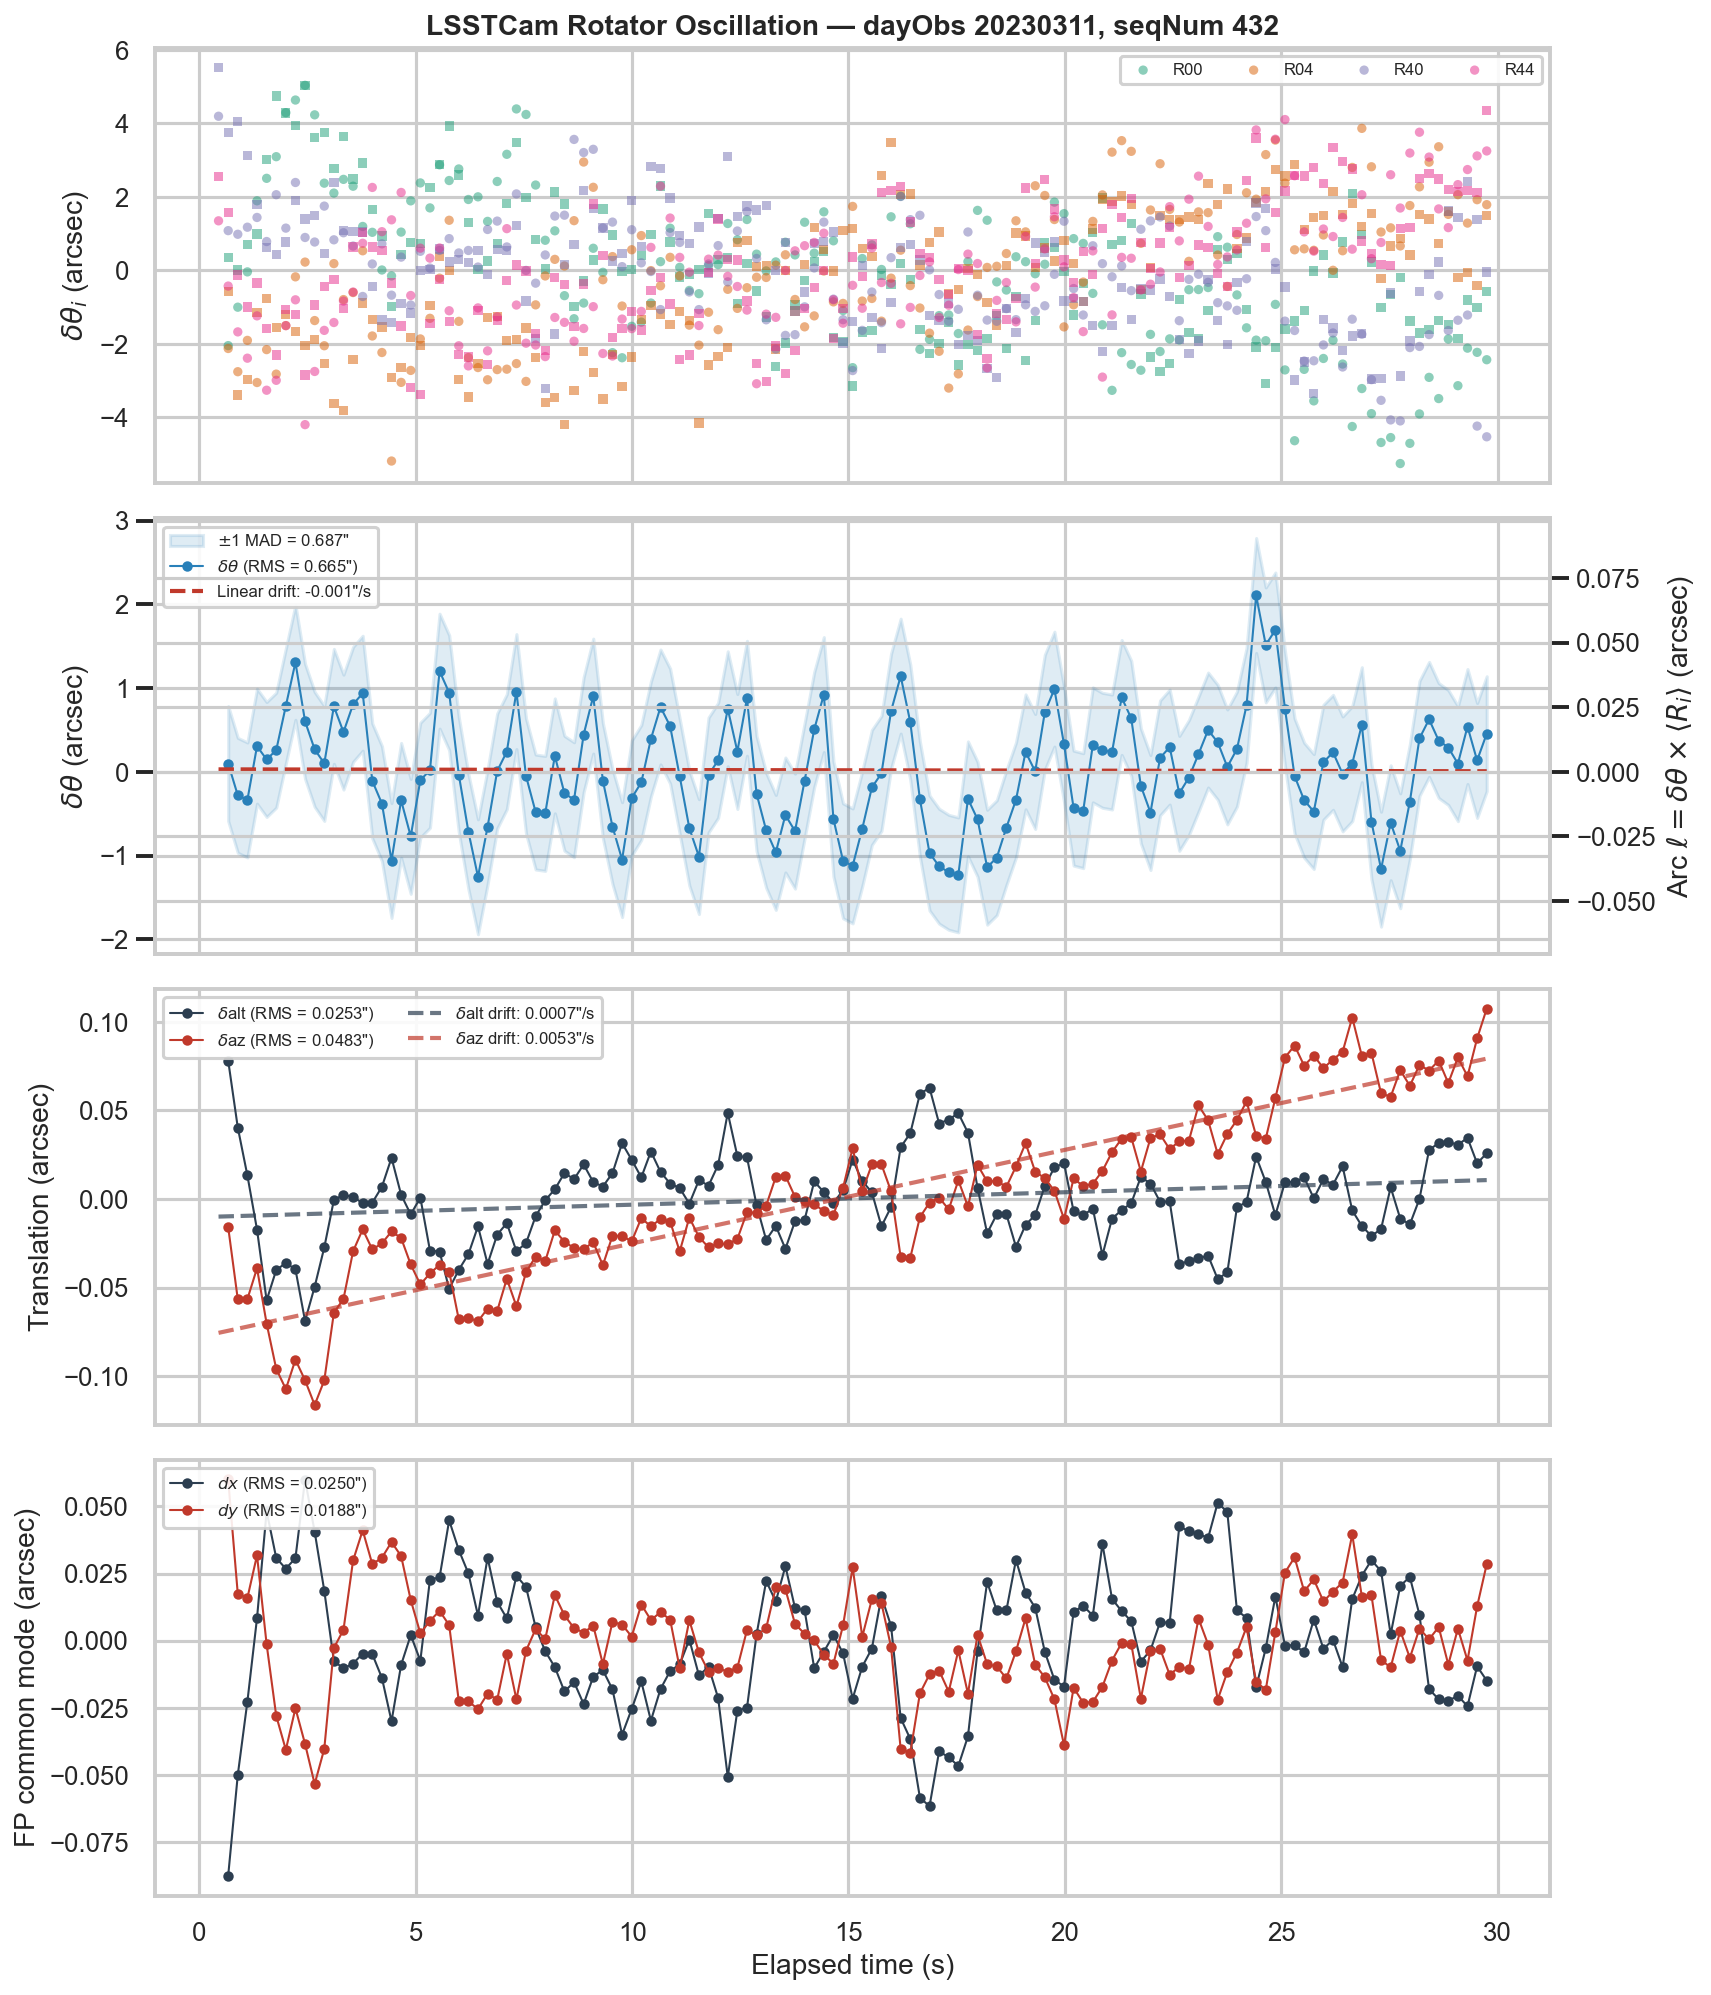
\includegraphics[width=0.95\textwidth]{rotator_detrended.png}
\caption{Full decomposition of guider motions.  Panel~1: per-star
$\delta\theta_i$ from the 8 corner guiders.  Panel~2: rigid-body
$\delta\theta$ solution with $\pm 1$\,MAD noise band and linear drift.
Panel~3: common-mode translation in alt/az with linear tracking drift
fits.  Panel~4: focal-plane common-mode translation $(dx, dy)$ from
the per-frame hybrid fit (oscillatory rigid-body jitter after drift
removal).}
\label{fig:detrended}
\end{figure}

\clearpage
%======================================================================
\section{Summary}
\label{sec:summary}

\begin{itemize}
\item The displacement of each guide star is modelled as a rigid-body
  motion---common-mode translation $(dx, dy)$ plus rotation
  $\delta\theta$ about the optical axis---and a per-guider
  atmospheric/optical residual (Eq.~\ref{eq:displacement}).

\item Common-mode translations arise in two distinct frames:
  focal-plane rigid-body motions (rotator shift, flexure) are common
  in focal-plane coordinates, while the tracking drift is common in
  alt/az.  A purely alt/az model conflates the two; we therefore adopt
  a hybrid approach (Section~\ref{sec:hybrid_model}) that fits
  per-frame translations in the focal plane and models the tracking
  drift via per-guider $\mathbf{J}_i^{-1}$ mappings
  (Eq.~\ref{eq:hybrid_model}).

\item The linear tracking drift is incorporated directly into the
  augmented design matrix (Eq.~\ref{eq:augmented_A}), where the
  $\mathbf{J}_i^{-1}$ coefficients vary across guiders, providing the
  leverage to separate sky-frame drift from focal-plane motions.
  Per-frame residuals are then fit with the standard focal-plane
  design matrix for $(dx, dy, \delta\theta)$.

\item The rigid-body parameters are estimated using a robust
  M-estimator (Tukey bisquare loss with IRLS), which downweights
  guiders affected by anomalous atmospheric conditions or measurement
  artefacts.

\item For the analysed exposure, the rotator oscillation has RMS
  $0.767''$ with a dominant period of ${\sim}\,2$--$3$\,s, consistent
  with servo hunting.  At the mean guider radius
  $\langle R_i \rangle = 333$\,mm, this corresponds to a tangential
  arc of $\ell = \delta\theta \times \langle R_i \rangle$ with RMSE
  $= 0.025''$ and peak-to-peak $= 0.117''$, contributing directly to
  PSF elongation in the tangential direction at the focal plane edge.
\end{itemize}

\appendix

\section{Acknowledgements}

This material is based upon work supported in part by the National Science Foundation through Cooperative Agreements AST-1258333 and AST-2241526 and Cooperative Support Agreements AST-1202910 and AST-2211468 managed by the Association of Universities for Research in Astronomy (AURA), and the Department of Energy under Contract No.\ DE-AC02-76SF00515 with the SLAC National Accelerator Laboratory managed by Stanford University.
Additional Rubin Observatory funding comes from private donations, grants to universities, and in-kind support from LSST-DA Institutional Members.

% Include all the relevant bib files.
% https://lsst-texmf.lsst.io/lsstdoc.html#bibliographies
\section{References} \label{sec:bib}
\renewcommand{\refname}{} % Suppress default Bibliography section
\bibliography{local,lsst,lsst-dm,refs_ads,refs,books}

% Make sure lsst-texmf/bin/generateAcronyms.py is in your path
\section{Acronyms} \label{sec:acronyms}
\addtocounter{table}{-1}
\begin{longtable}{p{0.145\textwidth}p{0.8\textwidth}}\hline
\textbf{Acronym} & \textbf{Description}  \\\hline

AST & NSF Division of Astronomical Sciences \\\hline
AURA & Association of Universities for Research in Astronomy \\\hline
CD & Critical Design \\\hline
DE-AC02 & Department of Energy contract number prefix \\\hline
FITS & Flexible Image Transport System \\\hline
IRLS & Iteratively Reweighted Least Squares \\\hline
LSST-DA & LSST Discovery Alliance \\\hline
LSSTCam & LSST Science Camera \\\hline
MAD & Median Absolute Deviation \\\hline
OLS & Ordinary Least Squares \\\hline
PSF & Point Spread Function \\\hline
RMS & Root-Mean-Square \\\hline
RMSE & Root Mean Square Error \\\hline
SG0 & Segment Guide Sensor 0 \\\hline
SG1 & Segment Guide Sensor 1 \\\hline
SLAC & SLAC National Accelerator Laboratory \\\hline
WCS & World Coordinate System \\\hline
\end{longtable}

% If you want glossary uncomment below -- comment out the two lines above
%\printglossaries

\end{document}
